\documentclass[12pt]{article}

\usepackage{fullpage}
\usepackage{multicol,multirow}
\usepackage{tabularx}
\usepackage{listings}
\usepackage{pgfplots}
\usepackage[utf8]{inputenc}
\usepackage[russian]{babel}

% Оригиналный шаблон: http://k806.ru/dalabs/da-report-template-2012.tex

\begin{document}

\section*{Лабораторная работа №2\, по курсу дискрeтного анализа: Сбалансированные деревья}

Выполнил студент группы М8О-212Б-22 МАИ \textit{Мамонтов Егор}.

\subsection*{Условие}

\textbf{Вариант:} 1

Необходимо создать программную библиотеку, реализующую указанную структуру данных, на основе которой разработать программу-словарь.
В словаре каждому ключу, представляющему из себя регистронезависимую последовательность букв английского алфавита длиной не более 256 символов,
поставлен в соответствие некоторый номер, от 0 до 264 - 1. Разным словам может быть поставлен в соответствие один и тот же номер.

Программа должна обрабатывать строки входного файла до его окончания. Каждая строка может иметь следующий формат:
\begin{itemize}
    \item \texttt{+ word 34} — добавить слово «word» с номером 34 в словарь. Программа должна вывести строку «OK», если операция прошла успешно,
    «Exist», если слово уже находится в словаре.

    \item \texttt{- word} — удалить слово «word» из словаря. Программа должна вывести «OK», если слово существовало и было удалено,
    «NoSuchWord», если слово в словаре не было найдено.

    \item \texttt{word} — найти в словаре слово «word». Программа должна вывести «OK: 34», если слово было найдено; число, которое следует за «OK:»
    — номер, присвоенный слову при добавлении. В случае, если слово в словаре не было обнаружено, нужно вывести строку «NoSuchWord».

    \item \texttt{! Save /path/to/file} — сохранить словарь в бинарном компактном представлении на диск в файл, указанный парамером команды.
    В случае успеха, программа должна вывести «OK», в случае неудачи выполнения операции, программа должна вывести описание ошибки (см. ниже).

    \item \texttt{! Load /path/to/file} — загрузить словарь из файла. Предполагается, что файл был ранее подготовлен при помощи команды Save. В случае успеха, программа должна вывести строку «OK», а загруженный словарь должен заменить текущий (с которым происходит работа); в случае неуспеха, должна быть выведена диагностика, а рабочий словарь должен остаться без изменений. Кроме системных ошибок, программа должна корректно обрабатывать случаи несовпадения формата указанного файла и представления данных словаря во внешнем файле.
\end{itemize}

Различия вариантов заключаются только в используемых структурах данных:
\textbf{AVL дерево.}

\newpage
\subsection*{Метод решения}

Был реализован класс узла Node и класс AVL дерева. Эта структура данных предоставляет функционал для вставки, удаления, поиска данных, загрузки дерева из файла и сохранения дерева в файл.

% \newpage
\subsection*{Описание программы}

Класс \texttt{AVL\_tree} реализует сбалансированное дерево поиска. Поддерживает операции вставки, удаления, поиска, загрузки дерева из файла и сохранения дерева в файл.

Класс \texttt{Node} содержит в себе структуру узла.


\newpage
\subsection*{Дневник отладки}

\begin{enumerate}
    \item Программа получила WA на тесте 1 в  "0. Декартово дерево". Проблема была в том, что я забыл учесть, что символы должны быть всегда прописными. Исправил это функцией tolow().
    \item Программа получила WA на тесте 5 в  "0. Декартово дерево". Проблема была в том, что я неверно написал работу балансировки дерева. Пришлось серьёзно переписывать дерево и узел.
    \item После исправления всех ошибок, программа прошла тесты "0. Декартово дерево".
    \item Программа с первого раза прошла все тесты "1. AVL-дерево".
\end{enumerate}

\newpage
\subsection*{Тест производительности}

Сложность вставки и удаления элементов в дереве $O(n log n)$, где n - количество узлов в дереве.
Сложность поиска элемента в дереве также $O(n log n)$.

Для построения графика (Рис. 1) использовались тесты с 10, 100, 250, 750, 1000, 2500, 5000, 7500, 10000, 25000, 50000, 75000, 100000 строками данных.
Из графика видно, что время работы сравнимо с временем работы \texttt{std::map}, но все же мой программа проигрывает в скорости.

\begin{figure}
    \centering
    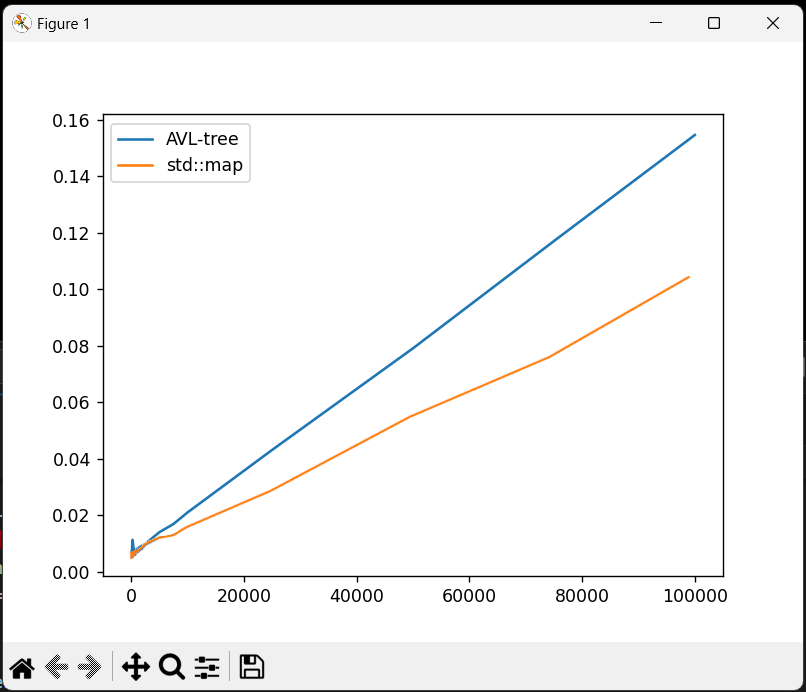
\includegraphics[width=\textwidth]{graph.png}
    \caption{График зависимости времени работы программы от количества введенных данных}
\end{figure}

\newpage
\subsection*{Выводы}

Сбалансированные деревья играют ключевую роль в хранении и поиске данных, обеспечивая быстрое выполнение операций вставки, поиска и удаления за логарифмическое время.
Это делает их особенно ценными для приложений, где требуется оперативный доступ к данным, таких как эффективные базы данных и ассоциативные массивы.
Однако создание и поддержание баланса в таких деревьях для операций вставки и удаления элементов может быть нетривиальной задачей.

\end{document}